\documentclass[10pt,a4paper]{article}

% ----- Paquetes -----
\usepackage[utf8]{inputenc}
\usepackage[T1]{fontenc}
\usepackage[spanish,es-nodecimaldot]{babel}
\usepackage[a4paper,top=1.8cm,bottom=1.8cm,left=2cm,right=2cm]{geometry}
\usepackage{amsmath,amssymb,amsfonts}
\usepackage{graphicx}
\usepackage{booktabs}
\usepackage{caption}
\usepackage{subcaption}
\usepackage{xcolor}
\usepackage[hidelinks]{hyperref}
\usepackage{authblk}
\usepackage{multicol}
\usepackage{siunitx}
\usepackage{placeins}

\captionsetup{font=small,labelfont=bf,justification=raggedright,singlelinecheck=false}
\setlength{\parindent}{0pt}
\setlength{\parskip}{0.5em}

% ----- Metadatos -----
\title{\vspace{-1.5em}Modelo fluido TCP/RED de Misra-Gomez-Towsley:\\
       aproximación numérica, análisis de estabilidad y bifurcación de Hopf}
\author{Abel Santiago García Ortiz\\
        \small Ingeniería de Sistemas e Informática\\
        \small \texttt{https://github.com/abel8000001/Proyecto-numerico}}
\date{\vspace{-1em}}

\begin{document}
\maketitle
\vspace{-2em}

% ============================================================================
\begin{abstract}
\noindent
\small
Se estudia el modelo fluido de Misra-Gomez-Towsley (MGT) que describe la
interacción no lineal entre el control de congestión TCP y el algoritmo
de gestión activa de colas RED en el cuello de botella de un router. El
sistema acopla tres ecuaciones diferenciales ordinarias (ventana TCP,
cola instantánea y promedio EWMA), no admite solución analítica cerrada
y exhibe una bifurcación de Hopf supercrítica al variar el peso $w_q$
del filtro RED. Se programan desde cero los métodos de Euler,
Runge-Kutta clásico de orden cuatro y Adams-Bashforth-Moulton
predictor-corrector de cuarto orden, validados contra
\texttt{solve\_ivp} (RK45). Las pendientes empíricas de convergencia
obtenidas son $1{,}04$, $3{,}76$ y $4{,}10$ respectivamente. Se
reproduce el equilibrio analítico con error relativo inferior al
$0{,}02\,\%$ y se caracteriza la bifurcación de Hopf en
$w_q^c = 1{,}06\times 10^{-2}$, con concordancia entre el análisis
lineal (autovalores del jacobiano) y la simulación no lineal del ciclo
límite emergente.
\end{abstract}
\vspace{-0.5em}

% ============================================================================
\section{Introducción}

Cuando una computadora envía datos por Internet (descargar un archivo,
ver un video, abrir una página web) no inyecta paquetes a la red de
forma arbitraria. El protocolo TCP (Transmission Control Protocol)
implementa un lazo cerrado de control. La fuente aumenta gradualmente la
cantidad de paquetes que envía sin esperar confirmación (la
\textit{ventana de congestión}), y cuando detecta que un paquete se
perdió, reduce esta ventana a la mitad. Es el principio de incremento
aditivo y decremento multiplicativo (AIMD). En el otro extremo del lazo
están los \textit{routers}, que cuando ven sus colas llenarse pueden
descartar paquetes para señalar congestión a las fuentes. El algoritmo
RED (Random Early Detection) hace esto con probabilidad creciente
conforme la cola crece, antes de que el buffer rebose. El resultado es
un sistema realimentado donde miles de fuentes y un router interactúan
continuamente, y cuyo comportamiento agregado puede modelarse con un
sistema de ecuaciones diferenciales: el modelo fluido propuesto por
Misra, Gomez y Towsley en SIGCOMM 2000~\cite{misra2000} (en adelante
modelo MGT).

Lo interesante del modelo es que, pese a ser determinista y de solo tres
ecuaciones, no admite solución analítica cerrada y exhibe un fenómeno
que se observa empíricamente en Internet real: cuando el parámetro de
promediado del router está mal ajustado, todas las fuentes TCP entran en
oscilaciones sincronizadas. Matemáticamente esto corresponde a una
\textit{bifurcación de Hopf}: un equilibrio estable que pierde
estabilidad y da lugar a un ciclo límite. Como ingeniero de sistemas
este fenómeno es relevante porque determina el desempeño efectivo de
cualquier aplicación distribuida (transferencias HTTP, video, bases de
datos remotas) que comparte un cuello de botella. La ausencia de
solución analítica se debe a cuatro razones: el término cuadrático
$W^2 p$ es no lineal; la curva $p(x)$ de RED es lineal por tramos; el
acoplamiento $W\to q\to x\to p\to W$ no es separable; y la formulación
rigurosa con retardo lo convertiría en una ecuación diferencial con
retardo. Por esto se requieren métodos numéricos.

Los objetivos del trabajo son: (i)~programar Euler, RK4 y
Adams-Bashforth-Moulton 4, validándolos contra \texttt{solve\_ivp};
(ii)~reproducir el equilibrio analítico y comparar el desempeño de los
métodos en términos de orden de convergencia y eficiencia computacional;
(iii)~caracterizar la bifurcación de Hopf al variar el peso EWMA $w_q$,
contrastando análisis lineal con simulación; (iv)~animar la dinámica
resultante. La sección~\ref{sec:metodologia} expone el modelo y los
métodos, la sección~\ref{sec:resultados} presenta los resultados con su
discusión, y la sección~\ref{sec:conclusiones} sintetiza los
aprendizajes.

% ============================================================================
\section{Metodología}
\label{sec:metodologia}

\subsection{Modelo matemático}

El estado del sistema queda descrito por tres variables: $W(t)$, la
ventana TCP promedio (cuántos paquetes pueden estar en vuelo
simultáneamente por flujo); $q(t)$, el tamaño instantáneo de la cola en
el router; y $x(t)$, una versión suavizada de $q$ obtenida mediante un
promedio móvil exponencial (EWMA), que es la que RED usa para tomar sus
decisiones. La formulación simplificada de Hollot, Misra, Towsley y
Gong~\cite{hollot2002}, que aproxima el retardo de ida y vuelta
$R\approx R_0$ por una constante, da:
\begin{subequations}
\label{eq:mgt}
\begin{align}
\frac{dW}{dt} &= \frac{1}{R} - \frac{W^2}{2R}\, p(x),\\
\frac{dq}{dt} &= -C + \frac{N\,W}{R}, \qquad q\geq 0,\\
\frac{dx}{dt} &= w_q\, C\,(q-x).
\end{align}
\end{subequations}

Cada término tiene una interpretación física directa. En (\ref{eq:mgt}a),
$1/R$ es la fase de incremento aditivo (la ventana sube en una unidad por
cada tiempo de ida y vuelta), mientras que $W^2 p / (2R)$ es el
decremento multiplicativo: cuando llega una marca de pérdida (que ocurre
con probabilidad $p$ sobre un flujo de tasa $W/R$), la ventana se reduce
a la mitad. En (\ref{eq:mgt}b), el router recibe paquetes a la tasa
agregada $NW/R$ (los $N$ flujos sumados) y los transmite a su capacidad
$C$; la diferencia es el ritmo al que crece o decrece la cola, con la
restricción física de que no puede ser negativa. En (\ref{eq:mgt}c), $x$
sigue a $q$ con una constante de tiempo $1/(w_q C)$: si $w_q$ es grande,
$x$ reacciona rápido y se parece a $q$; si $w_q$ es pequeño, $x$ alisa
las oscilaciones de $q$ a costa de reaccionar tarde. La curva de RED
relaciona $x$ con la probabilidad de descarte $p$:
\begin{equation}
p(x)=
\begin{cases}
0, & x\le q_{\min},\\
\dfrac{x-q_{\min}}{q_{\max}-q_{\min}}\,p_{\max}, & q_{\min}<x<q_{\max},\\
p_{\max}, & x\ge q_{\max}.
\end{cases}
\label{eq:red}
\end{equation}
Es decir, RED no descarta nada hasta que la cola promedio supera un
umbral mínimo $q_{\min}$, descarta de forma creciente hasta un umbral
máximo $q_{\max}$, y se mantiene en su máximo $p_{\max}$ por encima. Los
parámetros nominales (tabla~\ref{tab:params}) corresponden a un enlace
de 15~Mbps con paquetes de 500~B, valores publicados
en~\cite{hollot2002}.

\begin{table}[h]
\centering
\small
\caption{Parámetros del modelo MGT.}
\label{tab:params}
\begin{tabular}{lll}
\toprule
Símbolo & Significado & Valor nominal \\
\midrule
$N$ & Flujos TCP activos & $60$ \\
$C$ & Capacidad del enlace & $3750$ pkt/s \\
$R$ & RTT efectivo & $0{,}246$ s \\
$p_{\max}$ & Prob.\ máxima RED & $0{,}1$ \\
$q_{\min},q_{\max}$ & Umbrales RED & $150,\,700$ pkt \\
$w_q$ & Peso EWMA & variable \\
\bottomrule
\end{tabular}
\end{table}

\subsection{Reducción a primer orden y equilibrio analítico}

El sistema~(\ref{eq:mgt}) ya está en forma de primer orden, lo que es
conveniente porque todos los integradores numéricos esperan
$d\mathbf{y}/dt = \mathbf{f}(t,\mathbf{y})$ con $\mathbf{y}\in\mathbb{R}^n$.
El vector de estado es $\mathbf{y}=(W,q,x)^\top\in\mathbb{R}^3$ y
$\mathbf{f}(t,\mathbf{y})$ es el lado derecho de las tres ecuaciones.
Imponiendo $\mathbf{f}=\mathbf{0}$ (el sistema en reposo, sin cambios
temporales) se obtiene el punto de equilibrio en forma cerrada:
\begin{equation}
W^* = \frac{R\,C}{N},\quad
p^* = \frac{2N^2}{R^2 C^2},\quad
x^* = q^* = q_{\min}+\tfrac{p^*}{p_{\max}}(q_{\max}-q_{\min}).
\label{eq:eq}
\end{equation}
Con los valores nominales: $W^*=15{,}375$ pkt, $q^*=196{,}53$ pkt,
$p^*=8{,}46\times 10^{-3}$. Sustituyendo $\mathbf{y}^*$ en $\mathbf{f}$
se obtiene un residual de $2{,}66\times 10^{-15}$ (precisión de
máquina), lo que confirma la consistencia interna del modelo
implementado y sirve como primera prueba de validación del código antes
de cualquier integración numérica.

\subsection{Métodos numéricos}

Se programan tres métodos de paso fijo desde cero, con interfaz común
\texttt{integrator(f, t\_span, y0, h, args)}. Se usan tres
métodos para poder hacer comparaciones, pues cada uno representa un punto
distinto en el espacio precisión-vs-costo.

\begin{itemize}
\setlength{\itemsep}{0pt}
\item \textbf{Euler explícito} (orden 1): el esquema más simple posible,
$\mathbf{y}_{n+1}=\mathbf{y}_n + h\,\mathbf{f}_n$. Una sola evaluación
de $\mathbf{f}$ por paso. Sirve de referencia inferior.
\item \textbf{Runge-Kutta clásico} (orden 4): cuatro evaluaciones de
$\mathbf{f}$ por paso, distribuidas en el intervalo $[t_n, t_n+h]$.
Estándar de la industria para sistemas no rígidos.
\item \textbf{Adams-Bashforth-Moulton 4} (predictor-corrector PECE,
orden 4): primero un predictor explícito AB4 estima $\mathbf{y}_{n+1}$
usando los últimos cuatro $\mathbf{f}$, luego un corrector implícito AM4
lo refina evaluándose una sola vez. Total: dos evaluaciones de
$\mathbf{f}$ por paso, la mitad que RK4 a igual orden. El precio es
necesitar arranque con RK4 para los primeros tres pasos.
\end{itemize}

\subsection{Validación, herramientas y reproducibilidad}

La solución de referencia se obtiene con
\texttt{scipy.integrate.solve\_ivp} método RK45 (Dormand-Prince con
control adaptativo de paso) y tolerancias $\texttt{rtol}=10^{-10}$,
$\texttt{atol}=10^{-12}$~\cite{scipy}. Las métricas son el error global
$\|\mathbf{e}\|_\infty$ por componente, la pendiente empírica en escala
log-log y el número de evaluaciones de $\mathbf{f}$. Antes de aplicar
los integradores al modelo MGT se validó su orden sobre el oscilador
armónico (cuya solución es analítica): se obtuvieron pendientes
$1{,}01$, $4{,}00$ y $4{,}00$, en concordancia con la teoría; recién
después se aplicaron al sistema completo. Implementación en Python
(NumPy, SciPy, Matplotlib); el repositorio está organizado por módulos
(modelo, integradores, análisis, gráficas, animaciones) con scripts
reproducibles que regeneran todas las figuras del informe.

% ============================================================================
\section{Resultados y discusión}
\label{sec:resultados}

\subsection{Convergencia y eficiencia de los métodos}

Para una perturbación del 5\,\% sobre el equilibrio con
$w_q=5\times 10^{-2}$ (régimen estable), se midió el error global
$\|\mathbf{e}\|_\infty$ a $t=30$~s para cinco valores de $h$ entre
$5\times 10^{-3}$ y $2{,}5\times 10^{-4}$ (tabla~\ref{tab:convergencia}).
La \textit{pendiente empírica} se obtiene como la pendiente de la recta
que mejor ajusta los puntos $(\log h, \log\|\mathbf{e}\|_\infty)$ y debe
igualar el orden teórico del método. Las pendientes obtenidas son
$1{,}04$ (Euler), $3{,}76$ (RK4) y $4{,}10$ (ABM4), consistentes con los
órdenes 1, 4 y 4. RK4 cae ligeramente por debajo de 4 porque para $h$
pequeño su error se acerca al de la referencia adaptativa
($\sim 10^{-7}$) y satura.

\begin{table}[h]
\centering
\small
\caption{Convergencia empírica en el modelo MGT, $t\in[0,30]$~s,
perturbación inicial del 5\,\% sobre el equilibrio. $N_f$ es el número
total de evaluaciones de $\mathbf{f}$.}
\label{tab:convergencia}
\begin{tabular}{lrrr}
\toprule
Método & $h$ [s] & $\|\mathbf{e}\|_\infty$ & $N_f$ \\
\midrule
Euler & $5\times10^{-3}$ & $4{,}75\times10^{0}$  & 6\,000 \\
Euler & $1\times10^{-3}$ & $8{,}50\times10^{-1}$ & 30\,000 \\
Euler & $2{,}5\times10^{-4}$ & $2{,}08\times10^{-1}$ & 120\,000 \\
\multicolumn{4}{r}{Pendiente empírica: $1{,}04$} \\
\midrule
RK4   & $5\times10^{-3}$ & $5{,}25\times10^{-3}$ & 24\,000 \\
RK4   & $1\times10^{-3}$ & $4{,}46\times10^{-6}$ & 120\,000 \\
RK4   & $2{,}5\times10^{-4}$ & $1{,}02\times10^{-7}$ & 480\,000 \\
\multicolumn{4}{r}{Pendiente empírica: $3{,}76$} \\
\midrule
ABM4  & $5\times10^{-3}$ & $1{,}83\times10^{-2}$ & 12\,000 \\
ABM4  & $1\times10^{-3}$ & $1{,}65\times10^{-5}$ & 60\,000 \\
ABM4  & $2{,}5\times10^{-4}$ & $1{,}02\times10^{-7}$ & 240\,000 \\
\multicolumn{4}{r}{Pendiente empírica: $4{,}10$} \\
\bottomrule
\end{tabular}
\end{table}

\begin{figure}[!ht]
\centering
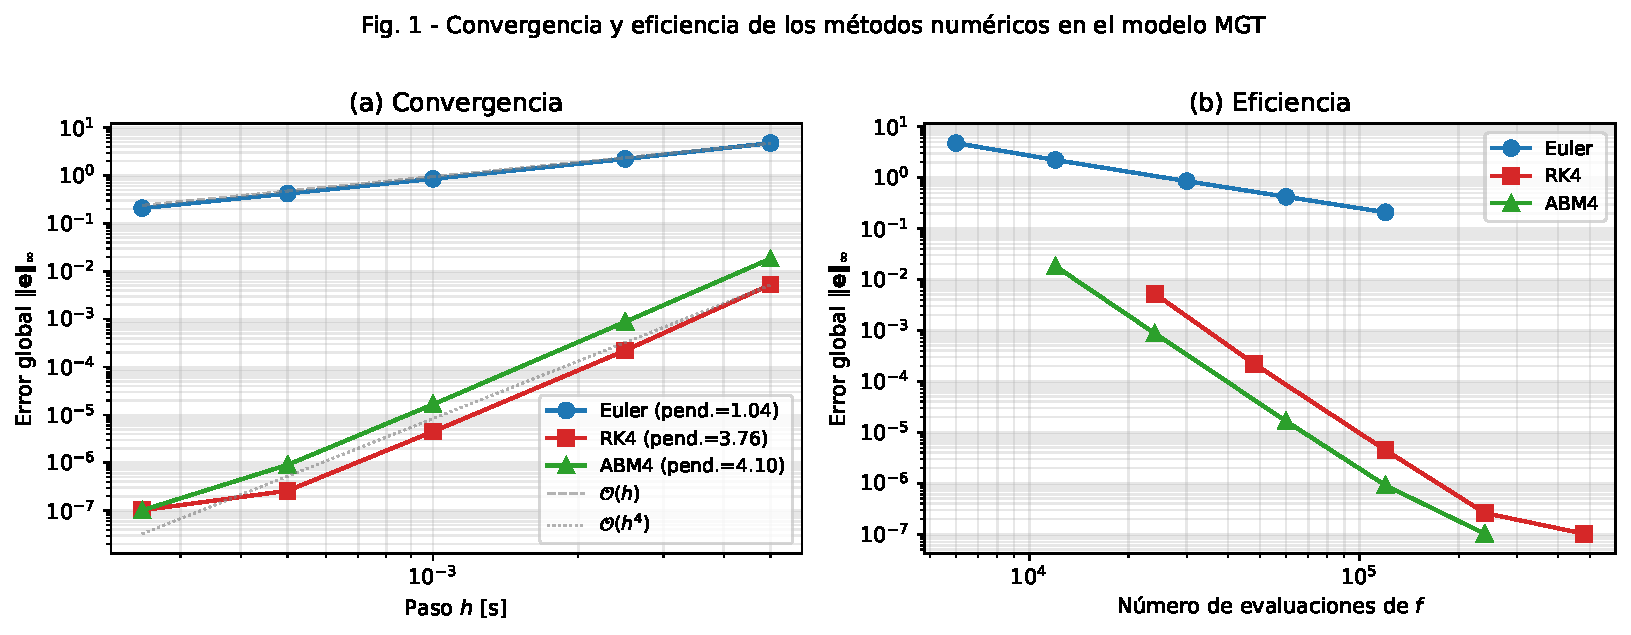
\includegraphics[width=0.76\linewidth]{figs/fig1_convergence.pdf}
\caption{Convergencia y eficiencia. (a)~Error global $\|\mathbf{e}\|_\infty$
vs.\ paso $h$ en escala log-log con pendientes teóricas
$\mathcal{O}(h)$ y $\mathcal{O}(h^4)$ como referencia. (b)~Error vs.\
número de evaluaciones de $\mathbf{f}$: a igual coste, ABM4 supera a RK4
por un factor $\sim 3$.}
\label{fig:convergencia}
\end{figure}

La figura~\ref{fig:convergencia}(b) muestra el lado más interesante de
la comparación: graficar el error contra el \textit{costo computacional}
(número de evaluaciones de $\mathbf{f}$) en lugar de contra $h$. A
igual costo, ABM4 es sistemáticamente más preciso que RK4 por un factor
cercano a 3. Esto justifica la elección del método multipaso: aunque
RK4 y ABM4 tienen el mismo orden teórico, ABM4 logra esa precisión con
la mitad de evaluaciones de $\mathbf{f}$ por paso en régimen.

Una limitación honesta del estudio: la curva $p(x)$ de RED es lineal por
tramos y por lo tanto no diferenciable en los umbrales $q_{\min}$ y
$q_{\max}$. Si la trayectoria cruza uno de estos umbrales durante la
simulación, los métodos de alto orden pierden su orden empírico (porque
los desarrollos de Taylor que sustentan RK4 y ABM4 requieren
diferenciabilidad). Para que la tabla midiera el orden teórico se
restringió la perturbación inicial al $5\,\%$, manteniendo la
trayectoria estrictamente dentro de la zona lineal de RED.
Adicionalmente, Euler explícito tiene un límite de estabilidad
$h_{\text{crit}}\approx 2/|\lambda_{\max}|=1{,}07\times 10^{-2}$~s
asociado al autovalor más rápido del sistema ($\lambda=-w_qC$, el modo
del filtro EWMA); para $h$ por encima de esta cota Euler diverge, una
manifestación clásica de la condición de estabilidad de los métodos
explícitos.

\FloatBarrier
\subsection{Régimen estable: convergencia al equilibrio}

Con $w_q=5\times 10^{-2}$ y perturbación inicial del 5\,\% sobre el
equilibrio, la simulación con RK4 a paso $h=10^{-3}$~s durante 30~s
converge al equilibrio analítico con error relativo de $0{,}010\,\%$ en
$W$ y $0{,}013\,\%$ en $q$ (figura~\ref{fig:estable}). La trayectoria
en el plano de fases $(W,q)$ es una espiral logarítmica con oscilaciones
amortiguadas que se reducen exponencialmente conforme el sistema
disipa la perturbación.

\begin{figure}[!ht]
\centering
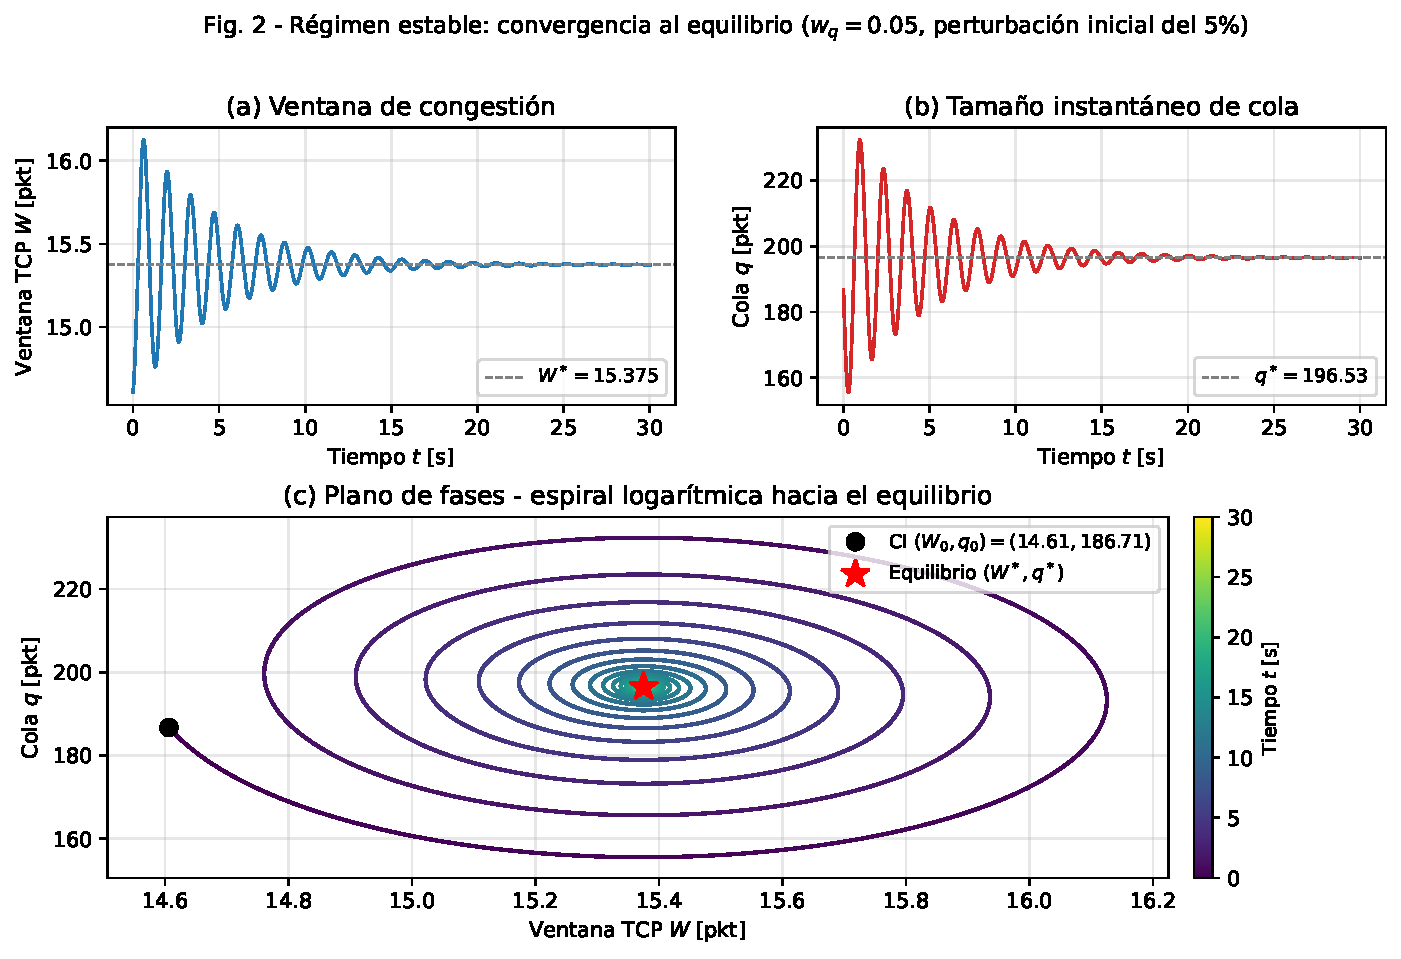
\includegraphics[width=0.76\linewidth]{figs/fig2_stable.pdf}
\caption{Régimen estable ($w_q=5\times 10^{-2}$, perturbación 5\,\%).
(a)~$W$ y (b)~$q$ convergen al equilibrio analítico.
(c)~Plano de fases: espiral hacia el punto fijo (estrella).}
\label{fig:estable}
\end{figure}

El periodo de las oscilaciones amortiguadas vale
$T_{\text{obs}}\approx 1{,}36$~s. Por otro lado, el análisis lineal del
sistema (ver §\ref{sec:hopf}) produce un par de autovalores complejos
conjugados $\lambda = -0{,}21 \pm 4{,}61j$, lo que predice un periodo
$T = 2\pi/\operatorname{Im}(\lambda) = 1{,}36$~s. La coincidencia (mejor
que $3\,\%$) entre el periodo observado en la simulación no lineal y
el predicho por el análisis lineal es la segunda prueba de validación:
el equilibrio y la frecuencia de las oscilaciones alrededor de él coinciden.

\FloatBarrier
\subsection{Bifurcación de Hopf supercrítica al variar \texorpdfstring{$w_q$}{wq}}
\label{sec:hopf}

Una \textit{bifurcación de Hopf} ocurre cuando, al variar un parámetro
del sistema, un equilibrio estable pierde su estabilidad y da paso a un
ciclo límite: una trayectoria cerrada y periódica que el sistema sigue
indefinidamente. Es \textit{supercrítica} cuando el ciclo emergente es
estable y nace con amplitud cero en el punto crítico, creciendo
suavemente conforme nos alejamos. Para detectarla numéricamente
linealizamos el sistema alrededor del equilibrio. Calculamos la matriz
jacobiana $J = \partial\mathbf{f}/\partial\mathbf{y}$ evaluada en
$\mathbf{y}^*$, sus autovalores son las tasas exponenciales de los
modos del sistema linealizado. Una parte real negativa indica que el
modo decae (estable), una positiva que crece (inestable), y una parte
imaginaria indica oscilación. Mientras todos tengan parte real
negativa, el equilibrio es estable; si uno cruza el eje imaginario, el
equilibrio bifurca.

Barriendo $w_q$ en escala logarítmica entre $10^{-6}$ y $10^{-1}$ y
calculando los autovalores de $J$ en cada caso, se localiza por
bisección un único cruce por cero de la parte real máxima en
$w_q^c = 1{,}060\times 10^{-2}$. En ese punto el espectro está
compuesto por un par complejo conjugado puro $\pm 4{,}586j$ y un real
puro $-40{,}29$. La firma característica de la bifurcación de Hopf es
precisamente esto, un par complejo cruzando el eje imaginario sin que
otros autovalores lo hagan. El tercer autovalor corresponde al modo
rápido del filtro EWMA y no participa de la bifurcación. La frecuencia
angular en el cruce predice un periodo del ciclo límite emergente de
$T_c = 2\pi/4{,}586 = 1{,}370$~s.

\begin{figure}[!t]
\centering
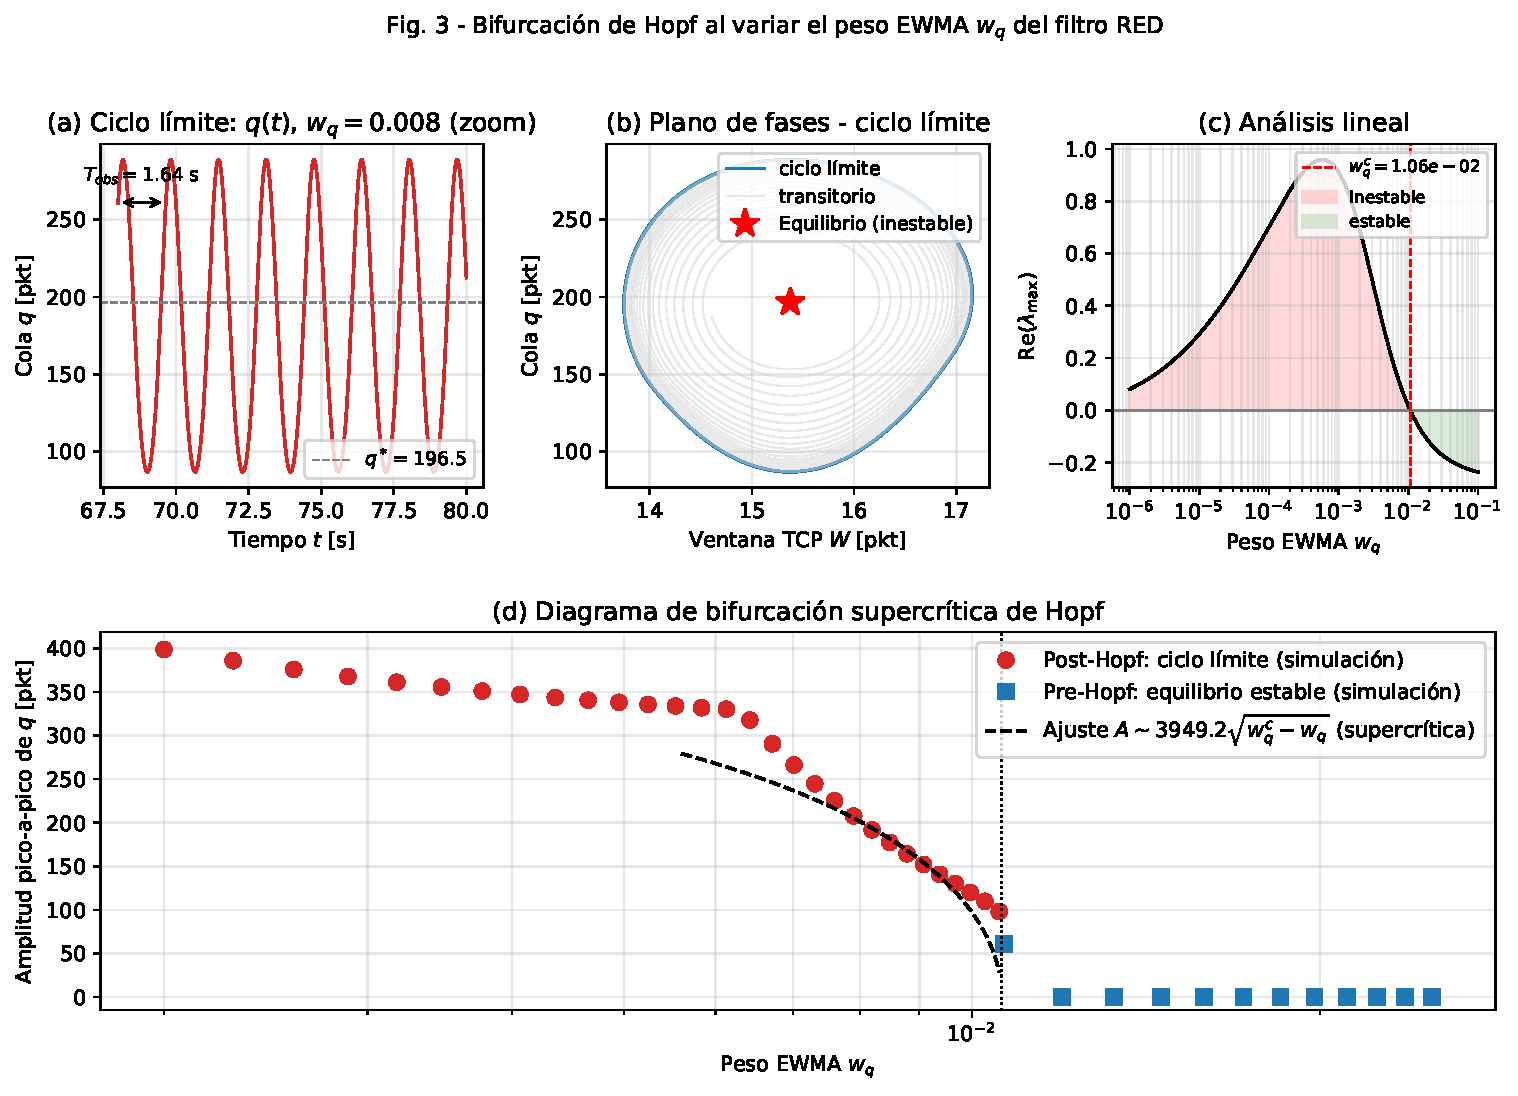
\includegraphics[width=0.72\linewidth]{figs/fig3_hopf.pdf}
\caption{Bifurcación de Hopf al variar $w_q$.
(a)~Ciclo límite estable en $q(t)$, $w_q=8\times 10^{-3}$.
(b)~Plano de fases: trayectoria espirala desde el equilibrio
(inestable) hacia el ciclo. (c)~Parte real máxima del jacobiano:
cruce por cero en $w_q^c=1{,}06\times 10^{-2}$.
(d)~Diagrama de bifurcación: amplitud pico-pico sigue
$A\sim\sqrt{w_q^c-w_q}$ cerca del punto crítico.}
\label{fig:hopf}
\end{figure}

En régimen post-Hopf con $w_q=8\times 10^{-3}$
(figura~\ref{fig:hopf}a, $\sim 25\,\%$ por debajo de $w_q^c$) la cola
oscila sostenidamente con periodo $T_{\text{obs}}=1{,}64$~s. La
discrepancia con la predicción lineal ($T_{\text{pred}}=1{,}38$~s) no
es un error: el análisis lineal solo describe oscilaciones de amplitud
infinitesimal, y aquí el ciclo tiene amplitud grande ($\sim 190$~pkt
pico-pico), régimen donde los términos no lineales del modelo
modifican apreciablemente la frecuencia. El panel (b) confirma esta no
linealidad mostrando un ciclo límite cerrado no exactamente elíptico.

El panel (d) es la verificación más completa. Para cada valor de $w_q$
se simuló el sistema hasta el atractor y se midió la amplitud
pico-pico de $q$ en estado estacionario. Cerca del punto crítico, los
puntos siguen $A\approx 3949\sqrt{w_q^c-w_q}$, ajustada por mínimos
cuadrados sobre los puntos no saturados. Esta dependencia de raíz
cuadrada es la ley universal de la Hopf supercrítica (proviene de la
forma normal del sistema) y su verificación numérica confirma que la
bifurcación es genuinamente supercrítica. Lejos del punto crítico la
rama se aplana cerca de $A\approx 340$~pkt, el ciclo límite toca la
saturación física $q\ge 0$ del modelo. Físicamente, $w_q$ pequeño
significa que RED promedia con constante de tiempo larga, introduciendo
un retardo efectivo en el lazo que produce las oscilaciones
sincronizadas reportadas en redes reales~\cite{floyd1993}. La
transición estable a ciclo límite al variar $w_q$ está documentada
en una animación con trazado simultáneo de $W(t)$, $q(t)$ y plano
de fases: \url{https://youtu.be/pxrYpyrs_wQ}.

% ============================================================================
\section{Conclusiones}
\label{sec:conclusiones}

Se reprodujo el equilibrio analítico con error relativo $<0{,}02\,\%$
y se confirmaron las pendientes empíricas $1{,}04$, $3{,}76$ y $4{,}10$
para Euler, RK4 y ABM4, con ABM4 superando a RK4 por factor $\sim 3$ en
eficiencia. Se caracterizó la bifurcación de Hopf supercrítica en
$w_q^c=1{,}06\times 10^{-2}$, un par complejo de autovalores cruza el
eje imaginario y emerge un ciclo límite con amplitud
$\sim\sqrt{w_q^c-w_q}$, conforme a la teoría de formas normales. 0\% del
contenido de este trabajo fue hecho por IA. Solo se usó IA para la investigación,
repaso de los temas y referencias del informe, y formateo del informe y presentación
en \LaTeX

% ============================================================================
\begin{thebibliography}{9}
\small

\bibitem{misra2000}
V.~Misra, W.-B.~Gong y D.~Towsley,
``Fluid-based analysis of a network of AQM routers supporting TCP flows with an application to RED,''
\textit{ACM SIGCOMM Computer Communication Review}, vol.~30, no.~4, pp.~151-160, 2000.

\bibitem{hollot2002}
C.~V.~Hollot, V.~Misra, D.~Towsley y W.-B.~Gong,
``Analysis and design of controllers for AQM routers supporting TCP flows,''
\textit{IEEE Trans.\ Automatic Control}, vol.~47, no.~6, pp.~945-959, 2002.

\bibitem{floyd1993}
S.~Floyd y V.~Jacobson,
``Random Early Detection gateways for congestion avoidance,''
\textit{IEEE/ACM Trans.\ Networking}, vol.~1, no.~4, pp.~397-413, 1993.

\bibitem{manjunath2019}
S.~Manjunath y G.~Raina,
``Compound TCP with Random Early Detection: stability, bifurcation and performance analyses,''
arXiv:1907.06302, 2019.

\bibitem{dormand1980}
J.~R.~Dormand y P.~J.~Prince,
``A family of embedded Runge-Kutta formulae,''
\textit{J.\ Comput.\ Appl.\ Math.}, vol.~6, no.~1, pp.~19-26, 1980.

\bibitem{hairer1993}
E.~Hairer, S.~P.~Nørsett y G.~Wanner,
\textit{Solving Ordinary Differential Equations I: Nonstiff Problems}.
Springer, 1993.

\bibitem{strogatz}
S.~H.~Strogatz,
\textit{Nonlinear Dynamics and Chaos}, 2.\textsuperscript{a}~ed.
Westview Press, 2015.

\bibitem{scipy}
P.~Virtanen \textit{et al.},
``SciPy 1.0: Fundamental algorithms for scientific computing in Python,''
\textit{Nature Methods}, vol.~17, no.~3, pp.~261-272, 2020.

\bibitem{rfc793}
J.~Postel,
``Transmission Control Protocol,''
RFC~793, IETF, 1981.

\end{thebibliography}

\end{document}
